\documentclass[conference]{IEEEtran}

% Packages
\usepackage{amsmath}
\usepackage{graphicx}
\usepackage{cite}
\usepackage{array}
\usepackage{booktabs}
\usepackage{url}
\usepackage{float}
\emergencystretch=3em

\begin{document}

\title{Validating Low Cost GNSS Bearing Estimation with Satellites in the Sky}

\author{
\IEEEauthorblockN{Parker Graham}
\IEEEauthorblockA{\textit{University of Colorado Boulder}}
}

\maketitle

% =========================
\begin{abstract}
Global Navigation Satellite Systems (GNSS) are increasingly affected by radio frequency interference (RFI), motivating low cost systems capable of detecting and localizing interference sources. Time difference of arrival (TDOA) methods have demonstrated strong performance for broadband GNSS interference, but continuous wave (CW) emitters provide limited timing observability. Angle of arrival (AoA) measurements are therefore a useful complementary observable for narrowband interference localization. This paper presents a satellite based validation method for a compact two element AoA receiver implemented with a USRP B210 operating at GPS L1. The method uses visible GPS satellites as calibration and validation sources because broadcast ephemeris provides known satellite azimuth and elevation, while measured inter channel carrier phase provides the projection of each satellite line of sight vector onto the antenna baseline. The resulting baseline vector estimate is used to evaluate whether the B210 can support repeatable two element AoA measurements for GNSS signals in the sky, forming a foundation for future CW interference bearing estimation.
\end{abstract}

% =========================
\section{Introduction}
Global Navigation Satellite Systems (GNSS) provide positioning, navigation, and timing (PNT) for aviation, maritime operations, communications, emergency services, financial timing, and other critical infrastructure. Civil GNSS signals arrive at the Earth's surface with extremely low received power, making them vulnerable to intentional and unintentional radio frequency interference (RFI) \cite{amin2016vulnerabilities,rados2024recent}. Recent aviation studies using ADS-B and flight data have reported widespread GNSS jamming impacts across Eastern Europe, the Black Sea region, and the eastern Mediterranean, demonstrating that GNSS RFI is an operational safety concern rather than a purely theoretical vulnerability \cite{felux2024impacts,figuet2022jamming}.

Localizing the source of interference is necessary for restoring healthy GNSS operations once an RFI event is detected. Gattis et al. demonstrated a real time TDOA system along the Polish coast of the Gulf of Gdansk that localized Baltic Sea jamming and spoofing sources using networked GNSS monitoring nodes \cite{gattis2026baltic}. That result shows the value of low size, weight, power, and cost (SWaP-C) monitoring systems in realistic interference environments. However, TDOA performs best when the received signal has sufficient timing structure or bandwidth. For continuous wave (CW) interference, timing observability is limited, making angle of arrival (AoA) an important complementary observable. Taylor et al. therefore proposed GNSS RFI localization through fusion of PDOA, TDOA, and AoA measurements, with AoA addressing cases where timing based methods are degraded \cite{taylor2024fusion}.

Multi antenna GNSS processing has also been studied extensively for interference mitigation. Chen et al. demonstrated real time GPS L1 C/A controlled reception pattern antenna (CRPA) processing in a software receiver, including satellite specific beam steering and MVDR processing \cite{chen2010realtime}. Live jamming tests also showed that CRPA receivers built from inexpensive general purpose components could provide practical GNSS robustness \cite{chen2013validation}. The present work is narrower than a full CRPA implementation as it validates the two channel phase observable required for compact AoA sensing.

The immediate motivation for this work comes from prior laboratory AoA testing with the KrakenSDR. The KrakenSDR is a five channel RTL SDR based receiver that uses a common clock, an internal noise source, and software correlation to estimate and correct per channel timing and phase offsets \cite{krakensdrDocs}. Correct bearing measurements were obtained after calibration, but the receiver had startup dependent channel phase biases, requiring recalibration after each power cycle. This behavior complicates field operation. The USRP B210 is considered here because it provides two receiver channels through the Analog Devices AD9361 transceiver and is advertised by Ettus Research as supporting coherent MIMO operation \cite{ettusB210,ad9361}. In contrast to the KrakenSDR observations, the B210 exhibited repeatable inter channel phase behavior across restarts, suggesting that a fixed calibration may remain valid unless the antenna geometry changes.

This paper validates the B210 AoA measurement concept using GPS satellites themselves as known signal sources. Satellite ephemeris provides the azimuth and elevation of each tracked satellite, allowing its line of sight vector to be computed in the local east-north-up (ENU) frame. Measured inter channel carrier phase differences are then used to estimate the effective antenna baseline vector. This approach directly tests whether the receiver preserves geometrically meaningful phase differences before introducing an unknown emitter.

% =========================
\section{Methodology}

\subsection{B210 USRP Recording}
The receiver front end uses two uBlox ANN-MB-00-00 multiband active GNSS antennas connected to the two receiver channels of an USRP B210. The antennas are separated by approximately $3.75$~in. ($0.095$~m), which is approximately one half wavelength at GPS L1. Since $\lambda = c/f_{L1}$ and $f_{L1}=1575.42$~MHz, the GPS L1 wavelength is approximately $0.190$~m, giving $\lambda/2 \approx 0.095$~m. In multi-antenna phased arrays, half-wavelength spacing is a vital constraint to prevent spatial aliasing. These ublox antennas also incorporate internal Low Noise Amplifiers (LNAs), which require a direct current (DC) bias voltage to operate. Thus, the signal path uses independent USB Bias Tee GP10 Labs modules, which inject the DC power into the radio frequency (RF) signal path to the active antennas. The RF outputs from the respective bias tees are routed directly into the Ettus Research USRP B210 via the physical ports labeled RF A RX2 and RF B RX2~\cite{ettusB210}. These physical ports are respectively mapped to Channel 0 and Channel 1.

The complete hardware configuration for this data collection is illustrated in Figure \ref{fig:b210_setup}.

\begin{figure}[h]
    \centering
    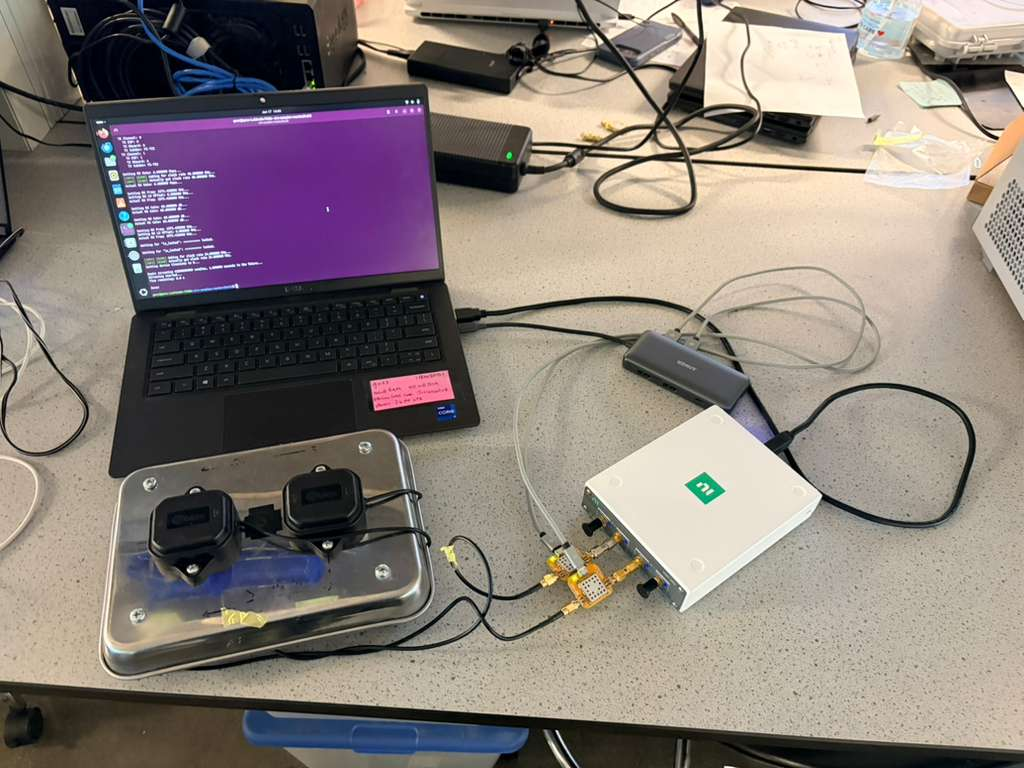
\includegraphics[width=\linewidth]{photos/b210_setup}
    \caption{Physical hardware setup including the USRP B210, dual ublox antennas on a metal plate, and GP10 Labs bias tees.}
    \label{fig:b210_setup}
\end{figure}

The data was captured using a Linux-based Ubuntu 26.04 laptop, which connected to the B210 via the Universal Hardware Driver (UHD) API over USB 3.0. The specific application used was \texttt{rx\_multi\_samples}, a UHD tool engineered for multi-channel streaming.

After first collecting 40 seconds of data from both antennas, the B210's USB was unplugged from the laptop, terminating power to the system. Then by waiting 10 seconds, which allows the SDR to thermally cool down and electrically stabilize, the hardware was reconnected, and another data set was captured. By comparing the phase differences between both antennas from both recording periods, the phase ambiguity of the USRP B210 can be evaluated.

Once the dual-channel binary files are written, the data is processed through a MATLAB-based SDR. This specific SDR implements a slaved correlator architecture, where the primary processing chain is from the first antenna data. This channel performs standard, full closed-loop tracking. The secondary channel, from the second antenna data, imports the exact code frequency, code phase, carrier frequency, and carrier phase generated by the first channel's NCO. By mathematically mixing the raw baseband signal from the second antenna with the replicas from antenna 1, the resulting In-phase ($I$) and Quadrature ($Q$) values represent the raw phase differential between the two antennas~\cite{chen2010realtime,chen2013validation}.

%____________the text below talks about the B210 architecture and why it is crucial for this specific application__________________

In modern SDRs, like the USRP B210, local oscillator (LO) frequencies are generated with Phase-Locked Loops (PLLs). Transceivers like the AD9361 use fractional-N synthesizers allowing for precise tuning to the L1 GPS frequency. When a fractional-N synthesizer is powered on, its internal digital divider networks initialize in a random state. If an SDR system relies on two separate synchronized RF chips, then though the two fractional-N PLLs will lock on to the correct frequency, their internal dividers however will start on a random phase. This results in a random static phase offset relative to one another. The USRP B210 bypasses this limitation because both receive channels are physically integrated into a single AD9361 circuit~\cite{ad9361}. This chip contains two identical main synthesizers, one dedicated to both transmitters, and one dedicated to both receivers. This single chip also shares the LO architecture for its receiving paths, which generates a singular LO waveform, then it is split and routed to the RX1 and RX2 ports~\cite{ad9361}. Since this splitting occurs after the PLL generation, the two receive channels are phase aligned, avoiding random phase ambiguities that other SDRs may experience.


\subsection{KrakenSDR Recording}

\begin{figure}[t]
\centering
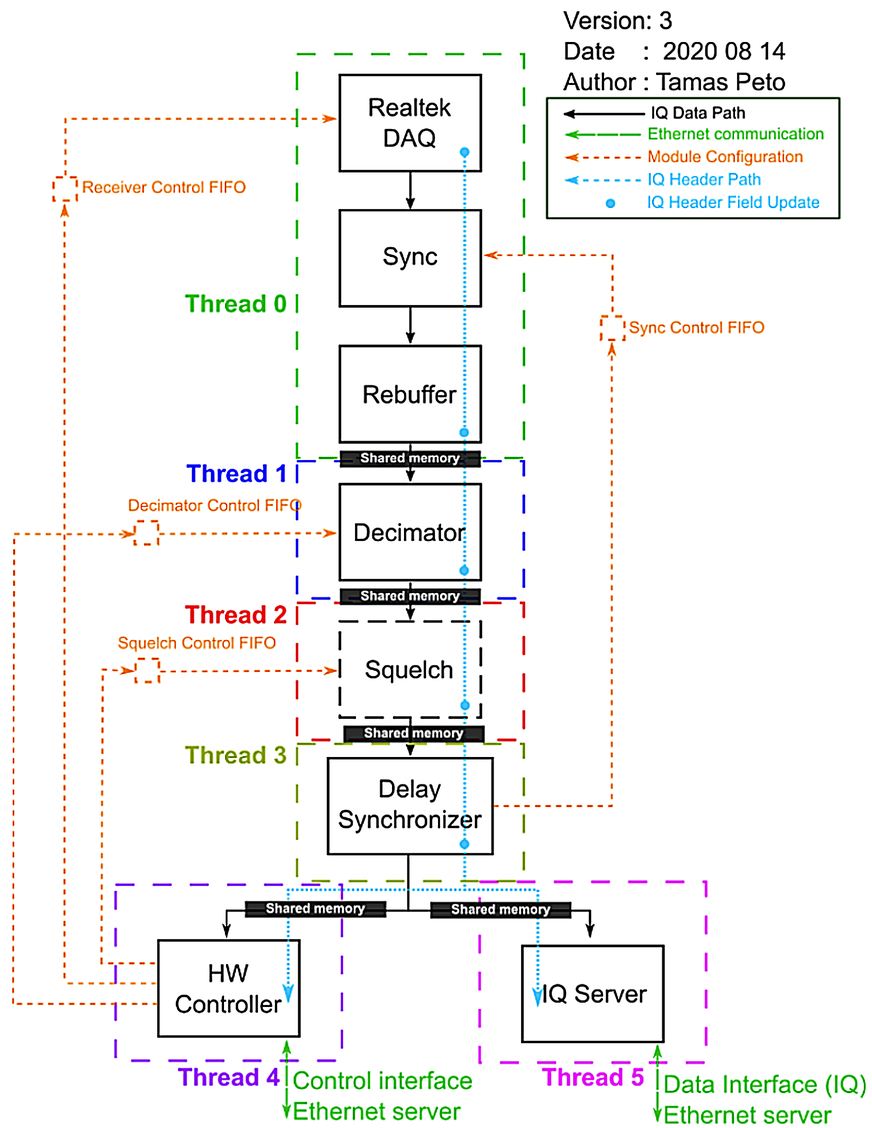
\includegraphics[width=0.85\linewidth]{photos/kraken_daq_sharpened_crisp.png}
\caption{KrakenRF/HeIMDALL data acquisition firmware architecture used for coherent multi-channel sample capture and startup calibration. Adapted from the HeIMDALL/Kerberos SDR DAQ documentation \cite{peto2020heimdall}.}
\label{fig:kraken_daq}
\end{figure}


KrakenSDR data was collected using the KrakenRF data acquisition software, which records raw $8$ bit I/Q samples from the receiver's five RTL-SDR channels. The DAQ architecture used for this workflow is shown in Fig.~\ref{fig:kraken_daq}. The Realtek DAQ block receives samples from each RTL-SDR and writes them to circular buffers. The downstream processing chain then re buffers the streams, applies decimation, and estimates residual inter channel delay, gain, and phase corrections using the receiver's internal calibration source. This startup calibration is required so that the five receiver channels share a common phase reference. Although the diagram is from the HeIMDALL/Kerberos SDR DAQ documentation, the Kerberos SDR and KrakenSDR use the same RTL-SDR based receiver architecture, with the primary hardware difference being that the Kerberos SDR provides four channels while the KrakenSDR provides five \cite{peto2020heimdall}. This runtime calibration is not required for the B210.

For this study, the KrakenRF software was used for calibrated recording rather than real time direction finding. After the DAQ software completed its startup calibration, the calibrated multi channel I/Q streams were saved for post processing. This preserved the channel alignment established by the KrakenSDR calibration procedure while allowing the recordings to be processed using the same phase bias and GNSS carrier phase analysis applied to the B210 data. 

\subsection{Phase Angle Difference Calculation}
The phase comparison is performed from the tracked prompt in phase and quadrature samples. For each selected PRN and time window, the master channel prompt components are first inspected as $I_P$ and $Q_P$, and the paired channel prompt components are inspected as $I_{PB}$ and $Q_{PB}$. The paired channel is then represented as a complex prompt sample sequence,

\begin{equation}
z_B[n] = I_{PB}[n] + jQ_{PB}[n].
\end{equation}

The raw phase angle for the paired channel is computed from the argument of this complex sequence and converted to degrees,

\begin{equation}
\phi_{\mathrm{raw}}[n] =
\frac{180}{\pi}\arg\left(z_B[n]\right).
\end{equation}

To match the analysis procedure used for the phase consistency check, negative phase values are shifted by $180^\circ$,

\begin{equation}
\phi_{\mathrm{adj}}[n] =
\begin{cases}
\phi_{\mathrm{raw}}[n] + 180^\circ, & \phi_{\mathrm{raw}}[n] < 0,\\
\phi_{\mathrm{raw}}[n], & \phi_{\mathrm{raw}}[n] \geq 0.
\end{cases}
\end{equation}

The adjusted phase sequence is then averaged over the selected time window to produce the reported phase angle for that PRN and collection. This procedure is applied consistently across the selected receiver channels so that the same phase-angle calculation can be compared across the test configurations.

\subsection{Test Configurations}
The test configurations are designed to compare inter channel phase behavior under three controlled collection conditions. Together, these configurations separate the effects of antenna geometry, receiver channel alignment, and static phase bias so that the B210 and KrakenSDR can be evaluated using the same general signal analysis where applicable.

The first configuration uses a two antenna array. For the B210, this configuration maps directly onto the two available receive ports, with one antenna connected to each channel. For the five channel KrakenSDR, two receiver ports are selected and grouped together for a given test. Treating the KrakenSDR as a two channel subset allows the same two antenna analysis to be applied to both receivers and provides a direct comparison against the B210 test configuration. INSERT PHOTO OF TWO ANTENNA ARRAY HERE

The second configuration uses a roof mounted antenna on the Anne J. Smead Aerospace Engineering Sciences building. In this configuration, the antenna output is split to the two receiver channels under test. The split antenna configuration is used for both the KrakenSDR and the B210, and the same signal analysis is performed on both receivers. This configuration provides a common input signal to the paired channels, which is useful for evaluating channel alignment without changing the downstream analysis method. INSERT PHOTO OF ROOF ANTENNA SPLIT HERE

The third configuration uses a signal generator input. This configuration is used only with the B210 and is intended to estimate the B210 inter channel phase bias. A controlled signal generator input is useful because the receiver channels can be driven by a known common signal, allowing the measured phase offset between the two channels to be interpreted as a receiver channel bias for that configuration.

\section{Results}

\subsection{Two Antenna Array Results}
The KrakenSDR two channel subset was evaluated using Sets~3 and~4, which were collected with the same selected channel pair before and after a power cycle. This configuration follows the same two channel structure used by the B210, allowing the KrakenSDR to be evaluated in a comparable two-port arrangement. The adjusted phase means for PRNs~5, 13, and 18 are summarized in Table~\ref{tab:kraken_two_channel_phase}. All three PRNs show substantial changes in mean phase between the two collections.

\begin{table}[h]
\centering
\caption{KrakenSDR adjusted phase means for selected PRNs}
\label{tab:kraken_two_channel_phase}
\begin{tabular}{cccc}
\toprule
PRN & Set 3 & Set 4 & Change \\
 & (deg) & (deg) & (deg) \\
\midrule
5  & 72.9 & 131.9 & +59.0 \\
13 & 51.0 & 122.3 & +71.3 \\
18 & 43.9 & 102.8 & +58.9 \\
\bottomrule
\end{tabular}
\end{table}

The B210 was evaluated using the same adjusted phase difference calculation for PRNs~10, 18, and 32. Figures~\ref{fig:b210_prn10_phase_cycle}--\ref{fig:b210_prn32_phase_cycle} show the sample phase difference before and after a B210 power cycle. Each figure includes the raw wrapped phase, the adjusted phase used in the analysis, and a horizontal line marking the adjusted mean reported in the plot title. The adjusted traces remain concentrated near their respective means over the selected processing window.

\begin{figure}[t]
\centering
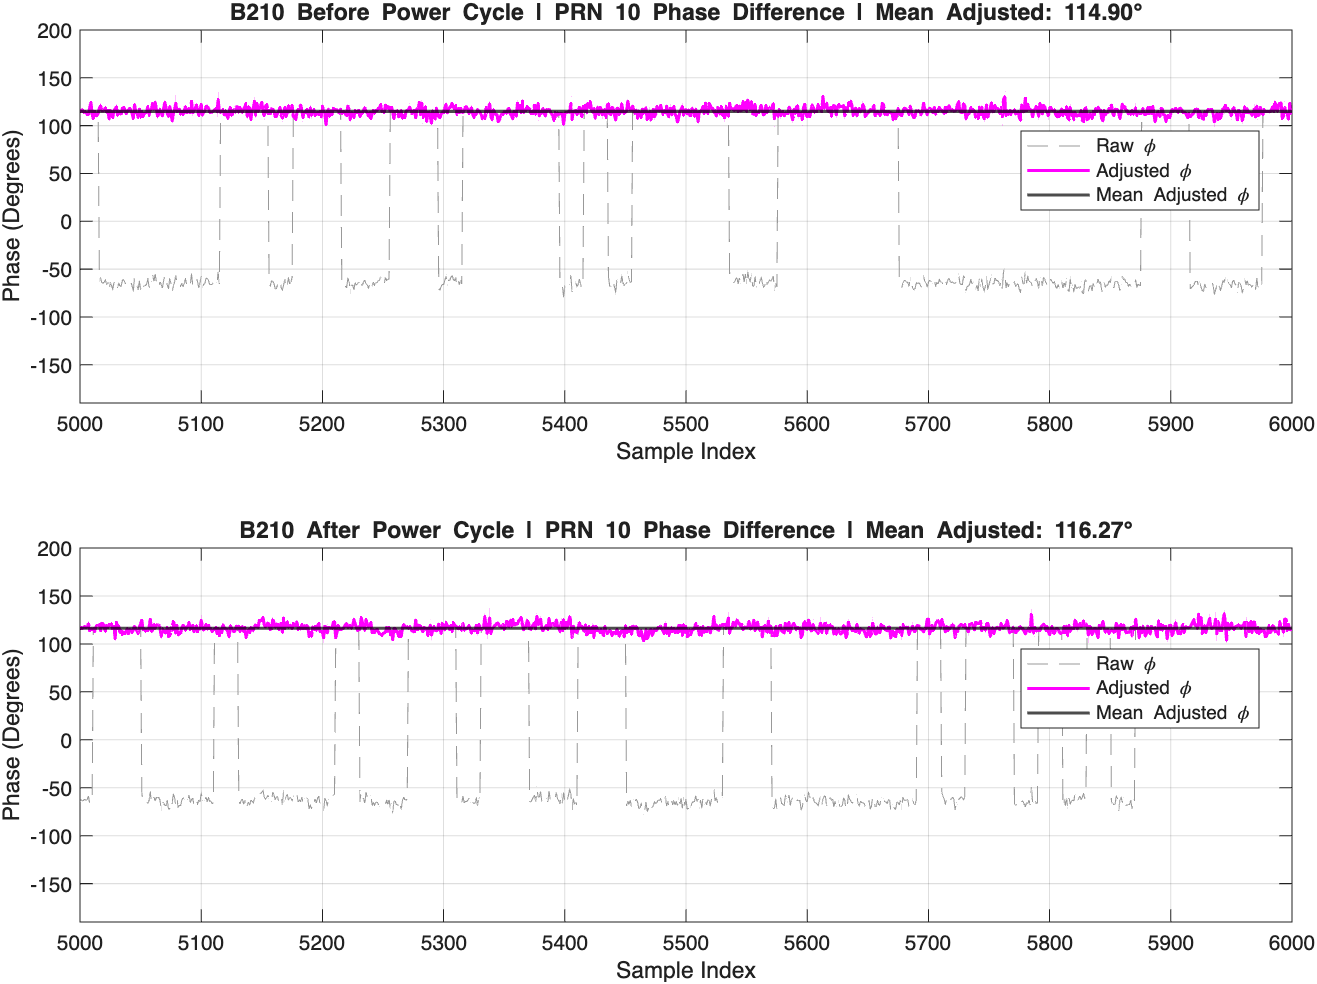
\includegraphics[width=\linewidth]{photos/prn10_phasediff.png}
\caption{B210 PRN~10 inter channel phase difference before and after the power cycle.}
\label{fig:b210_prn10_phase_cycle}
\end{figure}

\begin{figure}[t]
\centering
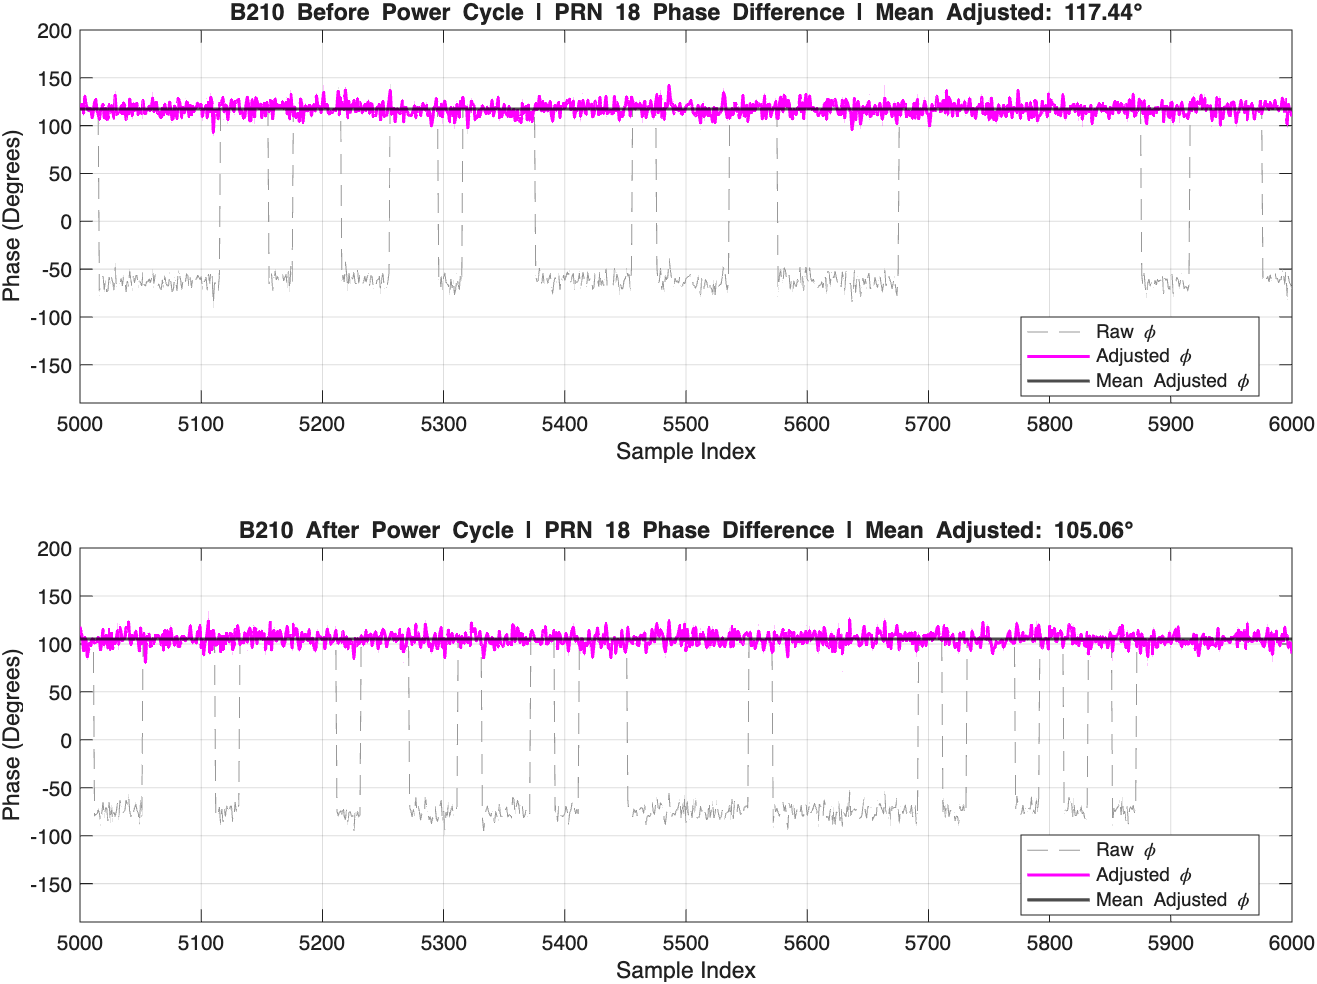
\includegraphics[width=\linewidth]{photos/prn18_phasediff.png}
\caption{B210 PRN~18 inter channel phase difference before and after the power cycle.}
\label{fig:b210_prn18_phase_cycle}
\end{figure}

\begin{figure}[t]
\centering
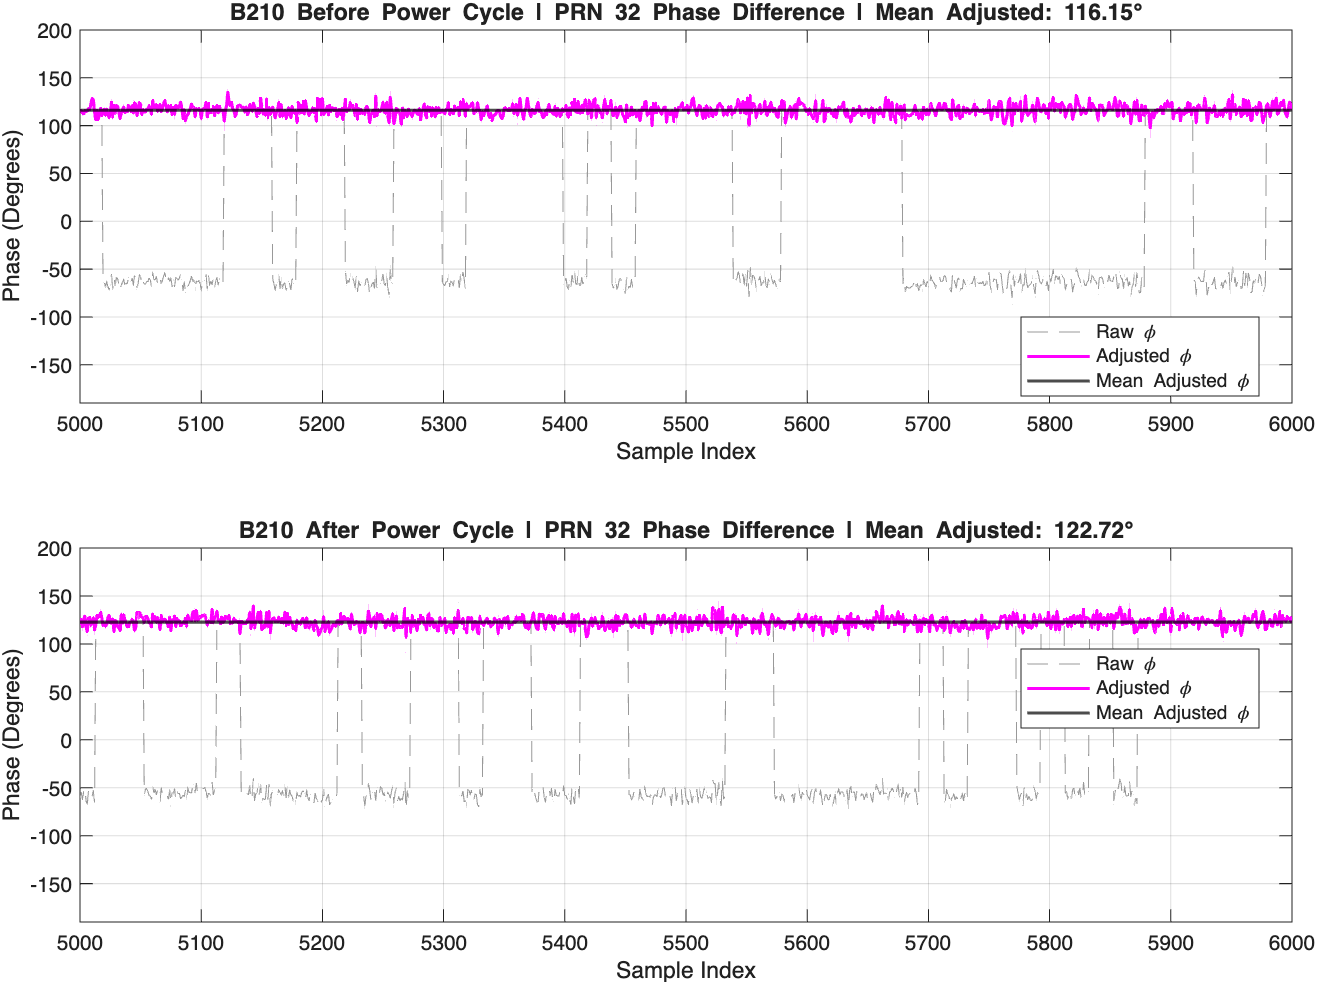
\includegraphics[width=\linewidth]{photos/prn32_phasediff.png}
\caption{B210 PRN~32 inter channel phase difference before and after the power cycle.}
\label{fig:b210_prn32_phase_cycle}
\end{figure}

The adjusted phase means shown in the B210 phase-difference plots are summarized in Table~\ref{tab:b210_two_channel_phase}. PRN~10 changed by $1.37^\circ$, PRN~32 changed by $6.57^\circ$, and PRN~18 showed the largest change at $12.38^\circ$ between the two collections.

\begin{table}[h]
\centering
\caption{B210 adjusted phase means for selected PRNs}
\label{tab:b210_two_channel_phase}
\begin{tabular}{cccc}
\toprule
PRN & Before Power Cycle & After Power Cycle & Change \\
 & (deg) & (deg) & (deg) \\
\midrule
10 & 114.90 & 116.27 &  +1.37 \\
18 & 117.44 & 105.06 & -12.38 \\
32 & 116.15 & 122.72 &  +6.57 \\
\bottomrule
\end{tabular}
\end{table}

\subsection{Split Roof Antenna Results}

To evaluate long-term hardware phase drift, the split roof antenna configuration was used for both the KrakenSDR and the USRP B210, which operated continuously for 120 minutes. Signal recordings consisting of one-minute snapshots were collected at three distinct intervals: $t=0$ minutes, $t=60$ minutes, and $t=118$ minutes. This configuration transmits a common physical signal from a single static antenna into a Mini-Circuits ZC4PD-18-S+ 4-way RF splitter; any measured carrier phase difference between the paired channels is a combination of the receiver's internal hardware bias and the phase unbalance of the splitter itself. According to the manufacturer's performance data, the ZC4PD-18-S+ has a phase unbalance of approximately $0.37^{\circ}-0.6^{\circ}$ near the $1575.42$ MHz GPS L1 frequency, with a maximum rated phase unbalance of $6.0^{\circ}$.

These datasets were processed through the slaved tracking architecture to compute the inter-channel carrier phase. The resulting phase means are summarized in Table IV. The KrakenSDR exhibited exceptional stability across the 2-hour window. Since the KrakenSDR utilizes an active, continuously tracking internal noise source to dynamically calibrate its RTL-SDR tuners, its mean phase difference remained around $114.7^{\circ}$ with standard deviations below $10^{\circ}$.

On the other hand, the USRP B210 relies on the physical stability of its shared AD9361 Local Oscillator without active digital recalibration. The results demonstrate thermal drift during continuous operation. The mean phase for PRN 15 drifted by nearly $20^{\circ}$ (from $98.76^{\circ}$ to $118.48^{\circ}$), while PRN 25 drifted by over $22^{\circ}$. Furthermore, the high standard deviations (approximately $80^{\circ}$) observed across the B210 PRNs suggest substantial intra-epoch phase noise or coherence degradation as the silicon components heated up. These results imply that while the B210 exhibits repeatable bias upon cold restarts (as evaluated in Section III-C), long-term continuous AoA deployments may require periodic recalibration or thermal stabilization.

\begin{table}[H]
\centering
\caption{LONG-TERM INTER-CHANNEL PHASE STABILITY (SPLIT ANTENNA)}
\begin{tabular}{lcccc}
\toprule
Receiver & PRN & $T=0$ min & $T=60$ min & $T=118$ min \\
         &     & Mean Bias & Mean Bias & Mean Bias \\
\midrule
KrakenSDR & 10 & $114.68^{\circ}$ & $115.02^{\circ}$ & $114.44^{\circ}$ \\
          & 15 & $114.54^{\circ}$ & $114.94^{\circ}$ & $113.66^{\circ}$ \\
          & 18 & $114.69^{\circ}$ & $114.90^{\circ}$ & $114.39^{\circ}$ \\
\midrule
USRP B210 & 5  & $121.63^{\circ}$ & $122.31^{\circ}$ & $111.77^{\circ}$ \\
          & 15 & $98.76^{\circ}$  & $109.60^{\circ}$ & $118.48^{\circ}$ \\
          & 25 & $119.13^{\circ}$ & $107.17^{\circ}$ & $96.74^{\circ}$  \\
\bottomrule
\end{tabular}
\end{table}

\subsection{Section 3.3}

It is also critical to note the tolerances of the Mini-Circuits ZAPD-2-2+ RF Splitter when testing the hardware bias. According to the manufacturer's performance data, the ZAPD-2+ splitter exhibits a typical phase unbalance of approximately $0.23^{\circ}$ near the $1575.42$ MHz GPS L1 frequency, with a maximum rated phase unbalance of up to $2.0^{\circ}$. Therefore, the measured phase offsets are partially due to the RF splitter.

\subsection{B210 Signal Generator Phase Bias Results}
The B210 splitter test was used to measure the static inter channel phase bias, denoted as $\phi_0$. In this configuration, the same RF signal is applied to both receiver channels, so the expected geometric phase difference is zero. Any remaining measured inter channel phase offset is therefore attributed to the receiver channel phase bias rather than antenna geometry.

The controlled splitter measurements showed that the B210 channel bias was repeatable across receiver restarts. A signal generator produced a sinusoidal test signal at GPS L1, which was divided with an RF splitter and applied to both B210 receive inputs. The B210 recorded both channels using the same multi channel receive configuration used for the satellite collections, so the measurement tested the phase repeatability of the receiver configuration used in the data collection.

Two repeatability checks were performed. In the first check, two recordings were separated by a full B210 power cycle. The measured phase bias changed from $-2.40^\circ$ to $-2.48^\circ$, a difference of $0.08^\circ$. In the second check, the receiver was operated for two hours before repeating the power cycle test. The measured phase bias changed from $-2.03^\circ$ to $-2.19^\circ$, a difference of $0.16^\circ$. These results, summarized in Table~\ref{tab:b210_bias_stability}, indicate that the mean inter channel phase bias remained stable at the sub degree level for the tested receiver configuration.

\begin{table}[h]
\centering
\caption{B210 splitter-measured inter channel phase bias repeatability}
\label{tab:b210_bias_stability}
\begin{tabular}{lccc}
\toprule
Condition & Mean Bias & Std. Dev. & Change \\
 & (deg) & (deg) & (deg) \\
\midrule
Initial recording & $-2.40$ & $2.10$ & -- \\
After power cycle & $-2.48$ & $2.12$ & $0.08$ \\
After two hour operation & $-2.03$ & $2.11$ & -- \\
After hot power cycle & $-2.19$ & $2.11$ & $0.16$ \\
\bottomrule
\end{tabular}
\end{table}

% =========================
\bibliographystyle{IEEEtran}
\bibliography{myBib}
\end{document}
